\section{Конструкторская часть}

В данном разделе рассматривается детализированная концептуальная модель системы. Описываются этапы создания невзаимозаменяемых токенов в блокчейн-сети, детали достижения консенсуса в сети, и алгоритм проверки подлинности сертификатов. Также приведены основные сценарии функционирования системы.

\subsection{Формализация задачи}

\subsubsection{Требования к разрабатываемую методу}
 
Для разрабатываемого метода создания уникальных сертификатов, подтверждающих окончание учебного заведения, предложен следующий список требований:
\begin{itemize}[leftmargin=1.6\parindent]
	\item[---] метод не должен допускать передачу сертификата другому пользователю;
	\item[---] только ограниченный пул участников может создавать сертификаты;
	\item[---] метод должен предоставлять возможность проверить подлинность сертификата;
	\item[---] во всех вычислительных узлах в один момент времени данные о выданных сертификатах не противоречат друг другу.
\end{itemize}


\subsubsection{Детализированная концептуальная модель системы}

Построенная IDEF0 диаграмма 1 уровня с декомпозицией решения исходной задачи, формализованной в разделе 1, представлена на рисунке \ref{fig:a3}. На данной схеме формализованная задача из раздела 1 была декомпозирована на подзадачи А1-3. В следующих подразделах даны описания алгоритмов каждой декомпозированной задачи.

\begin{figure}[!ht]
	\centering
	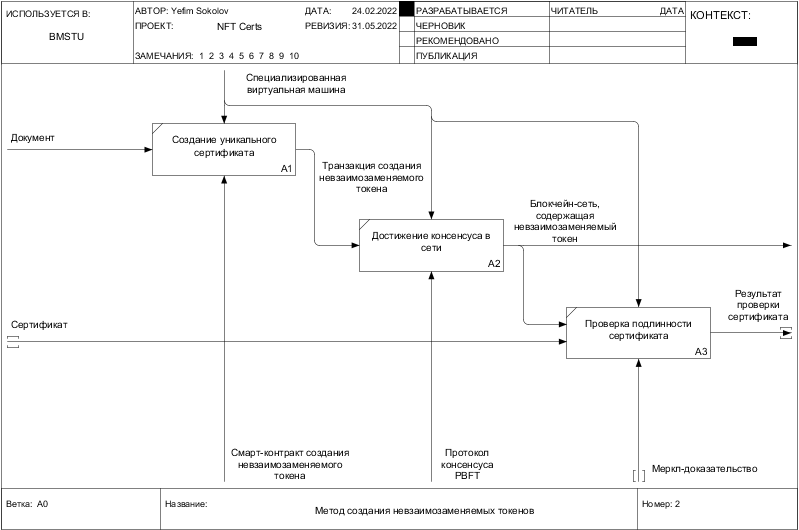
\includegraphics[width=\textwidth]{img/idef0_detail.png}
	\caption{Детализированная концептуальная модель системы в нотации IDEF0}
	\label{fig:a3}
\end{figure}

\subsection{Создание уникального сертификата}

Процесс создания уникального сертификата сводится к тому что, авторизованный на выдачу сертификатов участник (например, вуз) выполняет на специализированной виртуальной машине код смарт-контракта создания невзаимозаменяемого токена. Токен содержит в себе следующую информацию:
\begin{itemize}[leftmargin=1.6\parindent]
	\item[---] идентификатор сертификата (токена);
	\item[---] метаданные сертификата.
\end{itemize}
Идентификатором токена может быть целочисленное беззнаковое число, которое будет инкрементироваться для очередного сертификата, начиная с нуля или единицы. Под метаданными токена подразумевается полезная нагрузка, которая содержится в сертификате: ссылка на документ об окончании учебного заведения, наименование учебной организации и т.п. Заполнение метаданных токена - ответственность того, кто создает сертификат.

Факт выдачи сертификата заключается в том, что автор токена передает реципиенту идентификатор созданного сертификата, тем самым закрепляя факт владения сертификатом пользователем в сети.

Хранение в метаданных токена ссылки на документ, а не самого файла, и передача только идентификатора токена обусловлены тем, что блокчейн сеть - это одноранговая сеть, что подразумевает многократную репликацию данных в узлах сети. Таким образом, мы добиваемся снижения затрат на память и уменьшаем нагрузку на сеть.

На рисунке \ref{fig:a4} представлена схема алгоритма создания уникального сертификата.

\begin{figure}[hbtp]
	\centering
	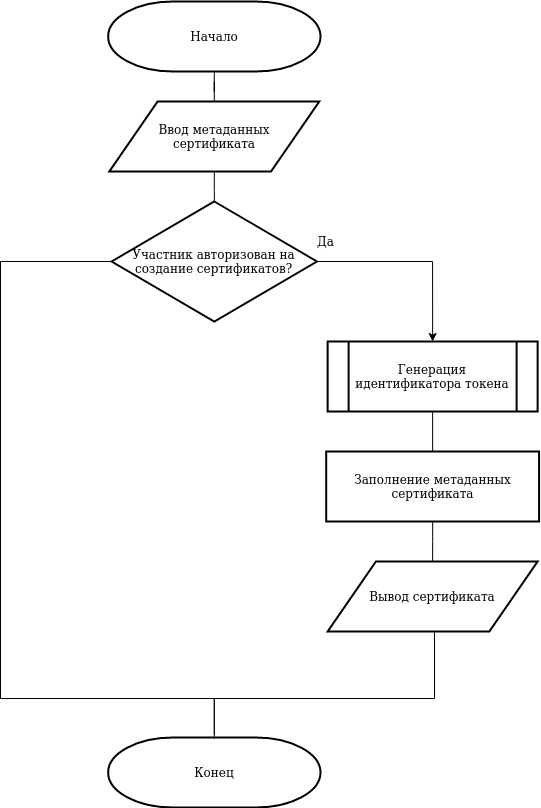
\includegraphics[width=\textwidth - 30pt]{img/create_nft.png}
	\caption{Алгоритм создания уникального сертификата}
	\label{fig:a4}
\end{figure}


\subsection{Достижение консенсуса в сети}

Задачу достижения консенсуса в распределенной сети разобьем на две подзадачи:
\begin{itemize}[leftmargin=1.6\parindent]
	\item[---] производство блоков;
	\item[---] финализация цепочек блоков (принятие решение о том, какая из ветвей блокчейна валидна).
\end{itemize}


\subsubsection{Производство блоков}

На основании проведенного в разделе 1 анализа, был сделан выбор в сторону алгоритма PBFT \cite{pbft}. Поскольку в PBFT новый блок сети создается в очередном раунде, разделим реальное время на дискретные слоты $s$ фиксированной длиной $t$ (индекс слота можно считать, как $\frac{t_{_{UNIX}}}{t}$). В каждый временной слот, только один участник (автор) может создать один и только один новый блок, автор блока выбирается как $s \bmod n$, где $n$ -- число авторизованных на создание блоков узлов.


\subsubsection{Финализация цепочек блоков}


Задача о финализации цепочек блоков заключается в детерминистическом принятии решения о том, какая из ветвей блокчейна является канонической, какие блоки являются подлинными, а не <<византийскими>>. В качестве протокола финализации был выбран протокол GRANDPA \cite{finality}.

Валидаторы протокола GRANDPA не создают блоки, а только голосуют за их цепочки. Таким образом, этот процесс может и должен происходить параллельно процессу производства блоков, то есть позволяет абстрагироваться от создания блоков, а также в будущем подменять алгоритм производства блоков, не изменяя протокол финализации.

Как и алгоритм PBFT, GRANDPA требует, чтобы <<честных>> валидаторов было как минимум две трети от их общего числа. Важным преимуществом данного протокола является его возможность за один раунд голосования финализировать более одного блока.


Предполагается, что распространение информации о новом блоком в сети не превышает длительность временного слота $t$. Если за время $t$ информация о новом блоке системы не дошла до всех участников сети, то возникают конкурирующие ветви блокчейн-сети, описанные в разделе 1. Чтобы разрешить конфликт ветвей, принято решение придерживаться правила более длинной ветви (англ. Longest chain rule) -- более длинная цепочка блоков считается валидной \cite{finality}. На рисунке \ref{fig:a5} приведен пример конфликта ветвей: черным отмечен уже финализированный блок, розовым -- <<лучшая>> (самая длинная) цепочка, серым -- блоки прочих веток.
\begin{figure}[hbtp]
	\centering
	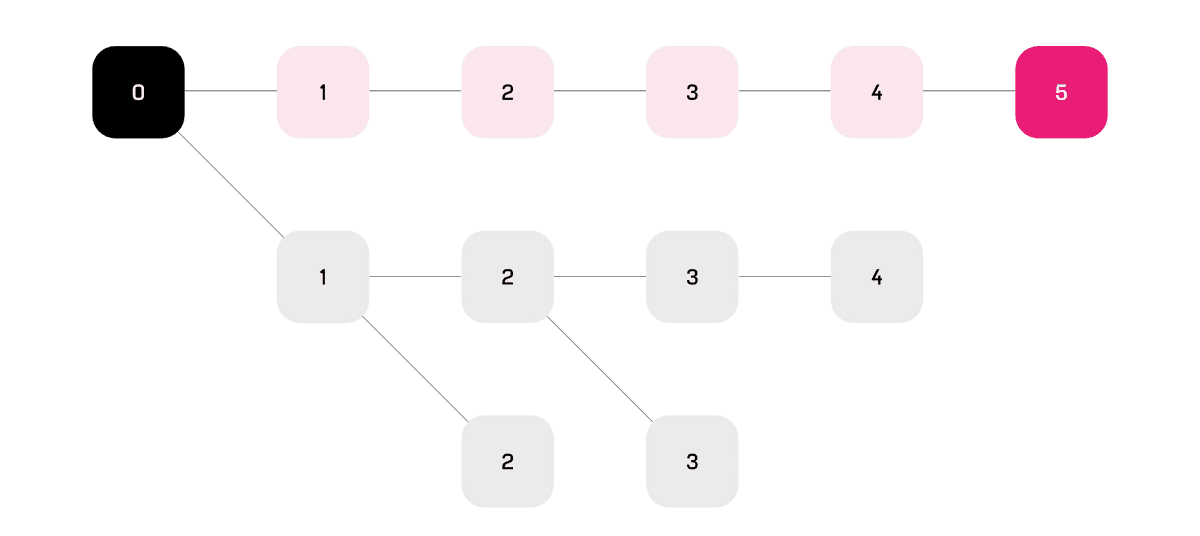
\includegraphics[width=\textwidth]{img/consensus_longest_chain.png}
	\caption{Разрешение конфликта ветвей}
	\label{fig:a5}
\end{figure}

Для обратной ситуации, когда в выделенный временной слот не было произведено блока, сеть может зависнуть, поскольку порядок авторов блоков строго регламентирован: автор $a$ будет ждать завершения автора $a-1$. Для решения этой проблемы, введем некоторый предельный период времени $T$. Если автор $a$ не дождется блока от автора $a-1$ за это время, то он в праве произвести собственный блок и цикл производства блоков возобновится.

Для своевременного достижения финализации сети, необходимо, чтобы узлы продолжали создавать блоки, даже если отсутствуют транзакции. Чтобы блокчейн-сеть не <<засорялась>> пустыми блоками, узлы могут отправлять <<пустое сообщение>> -- подписанный хэш текущего блока, тем самым не производя новый блок, но сохраняя консенсус в сети.


\subsection{Проверка подлинности сертификата}

Решение задачи проверки подлинности сертификата заключается в доказательстве существования блока в блокчейн-сети, в котором был создан проверяемый сертификат. Чтобы узел сети не скачивал все блоки сети, чтобы проверить факт вхождения, было принято решение воспользоваться деревом Меркла. 

Дерево Меркла - это сбалансированное бинарное дерево, в листьях которого содержатся хэши некоторых данных, причем в узлах вычисляется хэш от конкатенации хэшей узлов-потомков. Таким образом в корне дерева Меркл содержится хэш, в котором <<учтены>> все остальные хеши дерева. Такой корневой хэш, к тому же, учитывает порядок данных в листях дерева \cite{merkle}. Использование дерева Меркла позволяет хранить в узлах только корень дерева, который будет отражать всю историю транзакций в блокчейн-сети. На рисунке \ref{fig:a6} изображена иллюстрация дерева Меркла.

\begin{figure}[hbtp]
	\centering
	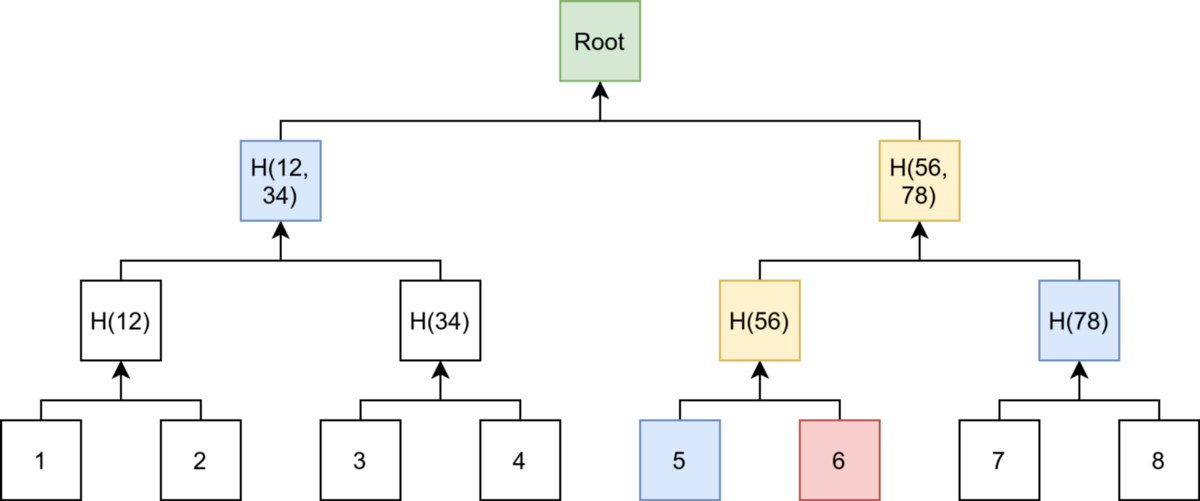
\includegraphics[width=\textwidth]{img/merkle_tree.png}
	\caption{Дерево Меркла}
	\label{fig:a6}
\end{figure}

Для выполнения проверки вхождения в дерево Меркла необходимо предоставить <<Меркл-докательство>> (англ. Merkle proof), которое является массивом хешей, размером $\log_{2}{N}$, где $N$ -- число листьев. Далее необходимо <<восстановить>> дерево Меркла: вычислить хэш от проверяемых данных, конкатенировать вычисленный хэш и хэш листа-брата, взятый из Меркл-доказательства, взять от результата конкатенации хэш и так далее вплоть до вычисления корневого хеша.
Подтверждением факта вхождения в дерево Меркла является равенство <<истинного>> и вычисленного хэша в корне дерева.

На рисунке \ref{fig:a7} представлена схема алгоритма доказательства включения в дерево Меркла.

\begin{figure}[hbtp]
	\centering
	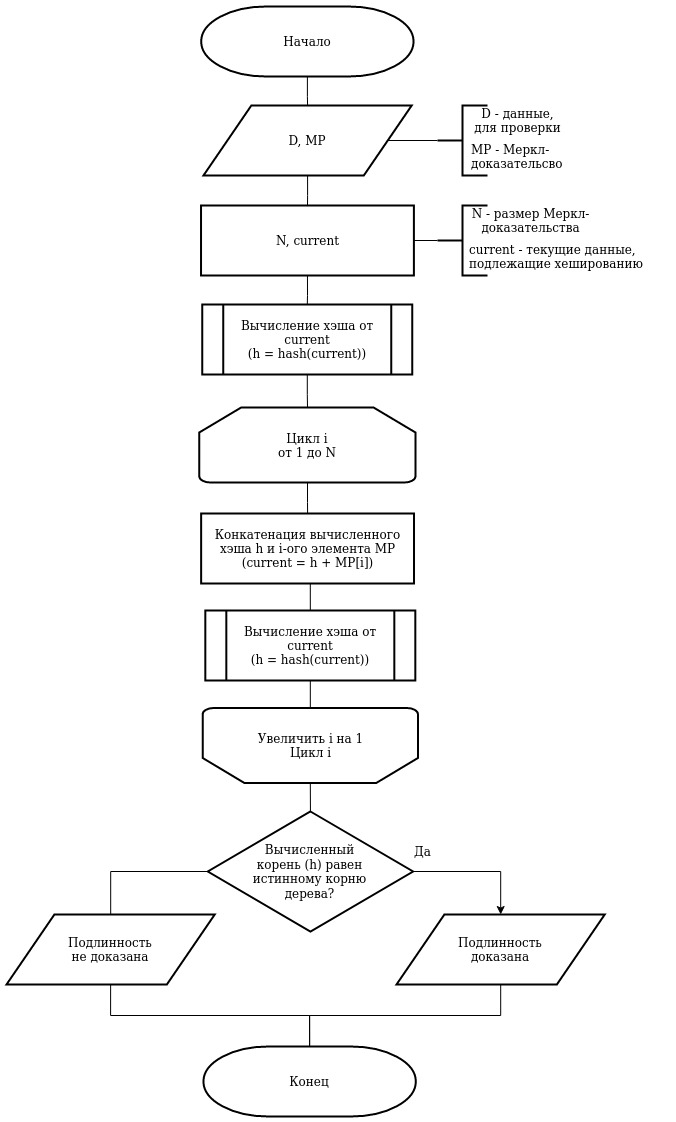
\includegraphics[height=\textheight - 40pt]{img/merkle_proof.png}
	\caption{Алгоритм доказательства включения в дерево Меркла}
	\label{fig:a7}
\end{figure}




\subsection{Сценарии функционирования системы}

Определим сценарии функционирования системы для наиболее часто используемых сценариев.

Сценарий для создания сертификата будет выглядеть следующим образом:
\begin{itemize}[leftmargin=1.6\parindent]
	\item[---] авторизованный на создание сертификатов участник сети (учебное заведение) производит невзаимозаменяемый токен в сети;
	\item[---] прочие авторизованные участники согласуют либо отвергают созданный сертификат;
	\item[---] если сертификат <<одобрен>> большинством, то он выдается пользователю (выпускнику учебного заведения).
\end{itemize}

Сценарий для проверки подлинности выданного сертификата будет выглядеть следующим образом:
\begin{itemize}[leftmargin=1.6\parindent]
	\item[---] выпускник предоставляет идентификатор своего сертификата;
	\item[---] участник сети получает подтверждение подлинности или фальшивости данного сертификата.
\end{itemize}


\subsection*{Выводы}
\addcontentsline{toc}{subsection}{Выводы}

Были представлены требования к разрабатываемому методу и детализированная концептуальная модель системы в нотации IDEF0. Приведены описание алгоритмов создания невзаимозаменяемых токенов, достижения консенсуса в сети и проверки подлинности сертификата. Приведены схемы разработанных алгоритмов.









%Пусть $SIGSET(B)$ -- множество подписей цепочки блоков B, полученных от других авторизованных узлов.
%\begin{equation}
%	SIGSET(B) = \{ a | \exists b \in B: AUTHOR(b) = a\}
%\end{equation}

%При условии если валидная цепочка $С$ оканчивается на $C[K..]$, где
%\begin{equation}
%	|SIGSET(C[K..])| > \frac{n}{2}
%\end{equation}
%Тогда $С[K..]$ и все его предки будут финализированы в сети.

%Определение финализации фактически базируется на большинстве голосов. В предложенной вариации %протокола консенсуса $2f+1 \le n$, где $f$ -- число византийских узлов. Таким образом, византийские %узлы не способны самостоятельно финализировать блоки.



%Список:

%\begin{itemize}[leftmargin=1.6\parindent]
%	\item[---] первое;
%	\item[---] второе;
%	\item[---] пятое;
%	\item[---] десятое.
%\end{itemize}

%Формула:

%\begin{equation}
%	c^2 = a^2 + b^2
%\end{equation}

%Ссылаемся на рисунок \ref{fig:a3}. Информация из источника \cite{golang}.


%\begin{code}
	%	\captionof{listing}{Пример кода}
	%	\label{code:1}
	%	\inputminted
	%	[
	%	frame=single,
	%	framerule=0.5pt,
	%	framesep=20pt,
	%	fontsize=\small,
	%	tabsize=4,
	%	linenos,
	%	numbersep=5pt,
	%	xleftmargin=10pt,
	%	]
	%	{text}
	%	{code/main.go}
	%\end{code}


\pagebreak